%For mobile and robotics applications a real-time encoder is needed. Hardware based real-time video encoders are expensive and not massively produced, thus their availability is limited. Creating one with off-the-shelf components opens the potential users. Two different models chosen whose computational cost was low enough to keep them operating at real-time and had kept biological plausibility constraints.


\subsection{General purpose computing in the GPU}

Some computer vision algorithms are parallel in nature and GPU architecture provides a good match for them. NVidia released \emph{compute unified device architecture} (CUDA) parallel programming model based on the work done for the \emph{Brook} extensions for the C language~\cite{buck2004brook,cuda}. This opened GPUs to general purpose programming. Years later, the Khronos Group unveiled OpenCL, which takes a CUDA-like approach to parallel programming (e.g. adds extensions to C and uses kernel calls). The main difference between them is that OpenCL may be used on other processing platforms (e.g. CPUs or FPGAs)~\cite{opencl}.

Since our retina modelling algorithms require 2D convolutions, and they can be performed in parallel, it was obvious that these could be performed on the GPU. One of the challenges to perform image convolution in the GPU is to move the required information between the different memory spaces defined in the OpenCL standard (Figure~\ref{fig:c2s:opencl-mem}). Sending an image from the host (usually a personal computer) to the Compute Device (in this case the GPU) is done through their global spaces; this memory type is normally has large capacity but is slow . 
From there the common practice is to process segments of the image in what is called a \emph{Compute Unit}, which hosts multiple computing cores or \emph{Work Items}. 
This segmentation permits the use of \emph{Local Memory}, which is visible only by the cores that belong to the Compute Unit. 
Access times from local memory are lower than from global memory but there are fewer bytes available for data. If the problem doesn't require much memory space, \emph{Private Memory} may be used for even faster than local memory access.

\begin{figure}[h]
  \begin{center}
    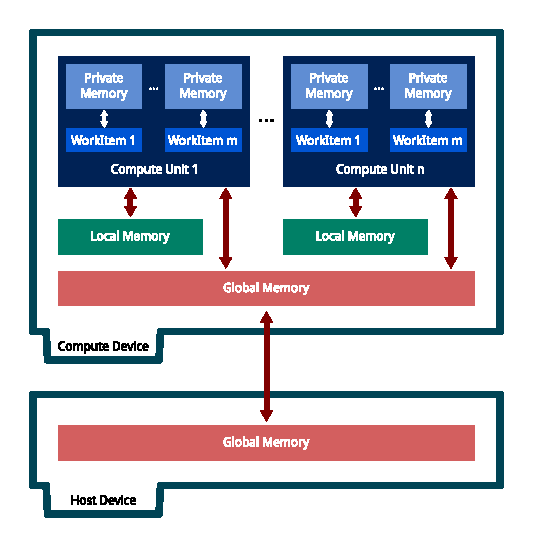
\includegraphics[width=0.6\textwidth]{opencl_memory}
    \caption{OpenCL memory hierarchy~\cite{opencl}.}
    \label{fig:c2s:opencl-mem}
  \end{center}
\end{figure}

OpenCL provides vector operations that may help increase the performance on some systems through Single Instruction-Multiple Data (SIMD) extensions in the computing cores\footnote{NVidia does not support them, while AMD and Intel do}. Programs that run on the device are known as \emph{kernels}, these are programmed using a subset of the C language. Each of the cores in the Compute Device will run the same kernel but may share data within its Compute Unit. Sharing data between Compute Units is done via global memory and it usually involves calling semaphores to ensure data coherency. Memory addresses are not protected but code may be prevented to write through atomic operations.

\subsection{Retina models}
\subsubsection{The foveal pit model}

The highest resolution area of the eye is the foveal pit (see Section~\ref{sec:vision:eye}). A functional model for this region of the retina was developed by \citeauthor{basab-model}, they called the implementation the \emph{Filter-overlap Correction algorithm} (FoCal)~\cite{basab-model}. It's based on the response and physiology of the fovea. The authors concluded that using four different layers of ganglion cells, most of the visually relevant information could be recovered after encoding. Furthermore, the encoder outputs a collection of rank-ordered spike trains. 

Ganglion cells where modelled using Difference of Gaussians (DoG, Equation~\ref{eq-dog}). 

\begin{equation}
\label{eq-dog}
DoG_w(x,y) = \pm\frac{1}{2\pi\sigma_{w,c}^2}e^{\frac{-(x^2 + y^2)}{2\sigma_{w,c}^2}}
\mp\frac{1}{2\pi\sigma_{w,s}^2}e^{\frac{-(x^2 + y^2)}{2\sigma_{w,s}^2}}
\end{equation}

The size of the receptive field of the simulated cells depends on the layer they belong to, this is reflected in the convolution kernel's width and parameters. Variables $\sigma_{w,c}$ and $\sigma_{w,s}$ are the standard deviation for the centre and surround components of the DoGs for layer $w$, respectively. The signs for the equation will be ($-$,$+$) if the ganglion cell is \textsc{off} centre and ($+$,$-$) if it is \textsc{on}centre. The parameters for this equation can be found in Table~\ref{tab-kernel-specs}.

\begin{table}[htb]
  \caption{Simulation parameters for ganglion cells}
  \centering
  \bgroup
  \def\arraystretch{1.4}
  
  %  \begin{TAB}(r,1em,1.5em){|c|c|c|c|c|}{|c|c|c|c|c|} 
  \begin{tabular}{c c c c c c}
    \begin{minipage}{1cm}Layer \end{minipage}& 
    \begin{minipage}{2cm}Behaviour \end{minipage}&
    \begin{minipage}{1cm} \centering Matrix width \end{minipage}&  
    \begin{minipage}{2.5cm}\centering Centre \\std. dev. ($\sigma_c$)\end{minipage} & 
    \begin{minipage}{2.5cm}\centering Surround \\std. dev. ($\sigma_s$)\end{minipage} & 
    \begin{minipage}{2.5cm}\centering Sampling resolution \\(cols, rows)\end{minipage} \\
    \hline
    \begin{minipage}{1cm}\vspace*{0.1cm} \centering1 \end{minipage} &
    \begin{minipage}{2cm}\textsc{off}-centre \vspace*{0.005cm} \end{minipage}& 
    \begin{minipage}{0.5cm}\centering$3$ \end{minipage}& 
    $0.8$ & $6.7 \times \sigma_c$ & 1, 1\\
    \begin{minipage}{1cm}\centering 2 \end{minipage} & 
    \begin{minipage}{2cm}\textsc{on}-centre \vspace*{0.005cm}\end{minipage} & 
    \begin{minipage}{0.5cm}\centering $11$ \end{minipage}& 
    $1.04$ & $6.7 \times \sigma_c$ &  1, 1\\
    \begin{minipage}{1cm}\centering 3 \end{minipage} &
    \begin{minipage}{2cm}\textsc{off}-centre \vspace*{0.005cm}\end{minipage} & 
    \begin{minipage}{1cm}\centering $61$ \end{minipage}& 
    $8$ & $4.8 \times \sigma_c$ & 5, 3 \\
    \begin{minipage}{1cm}\centering 4 \end{minipage} & 
    \begin{minipage}{2cm}\textsc{on}-centre \vspace*{0.005cm}\end{minipage} & 
    \begin{minipage}{0.5cm}\centering $243$\end{minipage} &
    $10.4$ & $4.8 \times \sigma_c$ & 5, 3
  \end{tabular}
  \label{tab-kernel-specs}
  \egroup
%  \vspace*{-5pt}
\end{table}

For each cell type, a convolution kernel must be computed and stored in a matrix ($DoG_{w}$). For each element in the matrix we use Equation~\ref{eq-dog}, substituting parameters specified in Table~\ref{tab-kernel-specs} and integer valued $x$-$y$ coordinates whose origin is the centre of the matrix. For example, for the $3\times3$ kernel (layer 1 cells), the upper-left value would be calculated as follows:

\begin{align}
\label{eq-dog-3x3}
DoG_3(x,y) &= -\frac{1}{2\pi\sigma_{3,c}^2}e^{\frac{-(x^2 + y^2)}{2\sigma_{3,c}^2}}
+ \frac{1}{2\pi\sigma_{3,s}^2}e^{\frac{-(x^2 + y^2)}{2\sigma_{3,s}^2}} \\
DoG_3(-1,-1) &= -\frac{1}{2\cdot\pi\cdot 0.8^2}e^{\frac{-((-1)^2 + (-1)^2)}{2\cdot 0.8^2}}
+ \frac{1}{2\cdot\pi\cdot 5.36^2}e^{\frac{-((-1)^2 + (-1)^2)}{2\cdot 5.36^2}} \nonumber \\[0.5em]
             &= 0.27399398 \nonumber
\end{align}

The procedure to encode images can be broken into two parts. First, Algorithm~\ref{code-focal-conv} simulates the ganglion cells. It requires four independent 2D convolutions (Eq.~\ref{eq-convolution}) using DoG kernels calculated as explained in previously. 

\begin{equation}
\label{eq-convolution}
C(x,y,w) = I \ast DoG_w = \sum_i \sum_j \left( I(i+x, j+y) \cdot DoG_w(i,j)\right)
\end{equation}

\begin{algorithm}[h]
  \caption{FoCal, Part 1}
  \label{code-focal-conv}
  \begin{algorithmic}
    \Procedure{GanglionCells}{image $I$, kernels $DoG$}
    \State $C \leftarrow \emptyset$
    \ForAll{$w \in Layers$}
    \State $C \leftarrow C \cup I \ast DoG_w$
    \EndFor
    \State \textbf{return} $C$
    \EndProcedure
    \algstore{bkbreak}
  \end{algorithmic}
\end{algorithm}

Pixel values that come out of the convolutions (Figures \ref{pic-lena-M-OFF}, \ref{pic-lena-M-ON}, \ref{pic-lena-P-OFF} and \ref{pic-lena-P-ON}) will be called coefficients. They are interpreted as quantities that are inversely proportional to the spike emission time. That is, the pixel with the largest coefficient value represents the ganglion cell that will spike first.

\begin{figure}[hbt]
  \centering
  \begin{subfigure}[t]{0.32\textwidth}
    \centering
    \captionsetup{justification=centering,margin=0.1cm}
    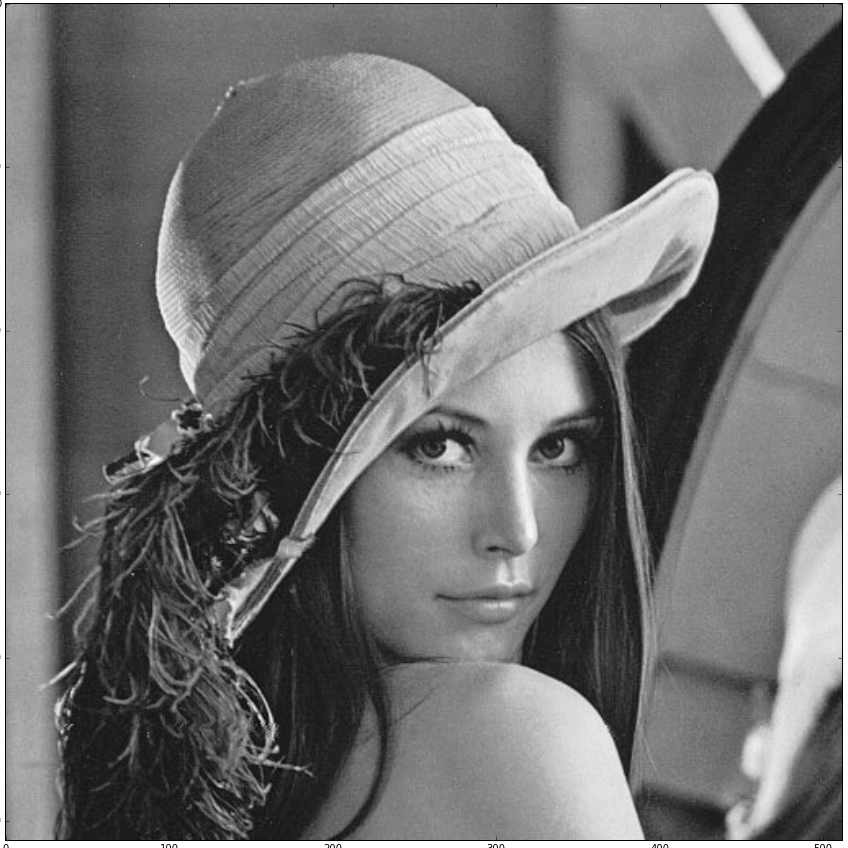
\includegraphics[width=\textwidth]{./Lena-gray}
    \caption{Original image}
    \label{pic-lena}
  \end{subfigure}
  \begin{subfigure}[t]{0.32\textwidth}
    \centering
    \captionsetup{justification=centering,margin=0.1cm}
    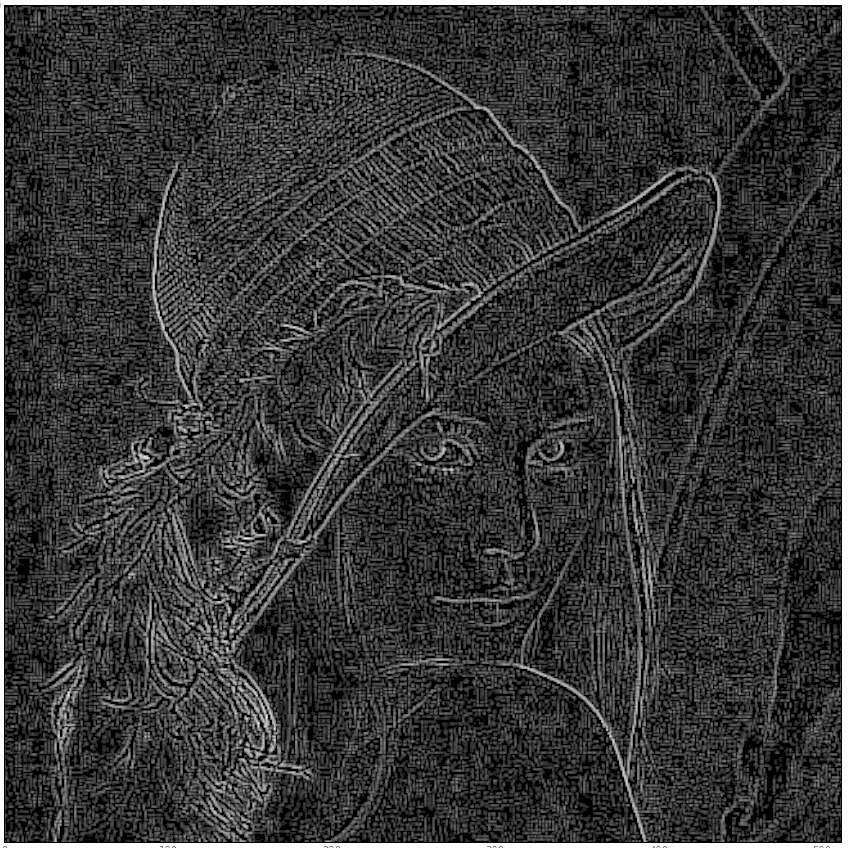
\includegraphics[width=\textwidth]{./Lena-midget_off}
    \caption{Layer 1}
    \label{pic-lena-M-OFF}
  \end{subfigure}
  \begin{subfigure}[t]{0.32\textwidth}
    \centering
    \captionsetup{justification=centering,margin=0.1cm}
    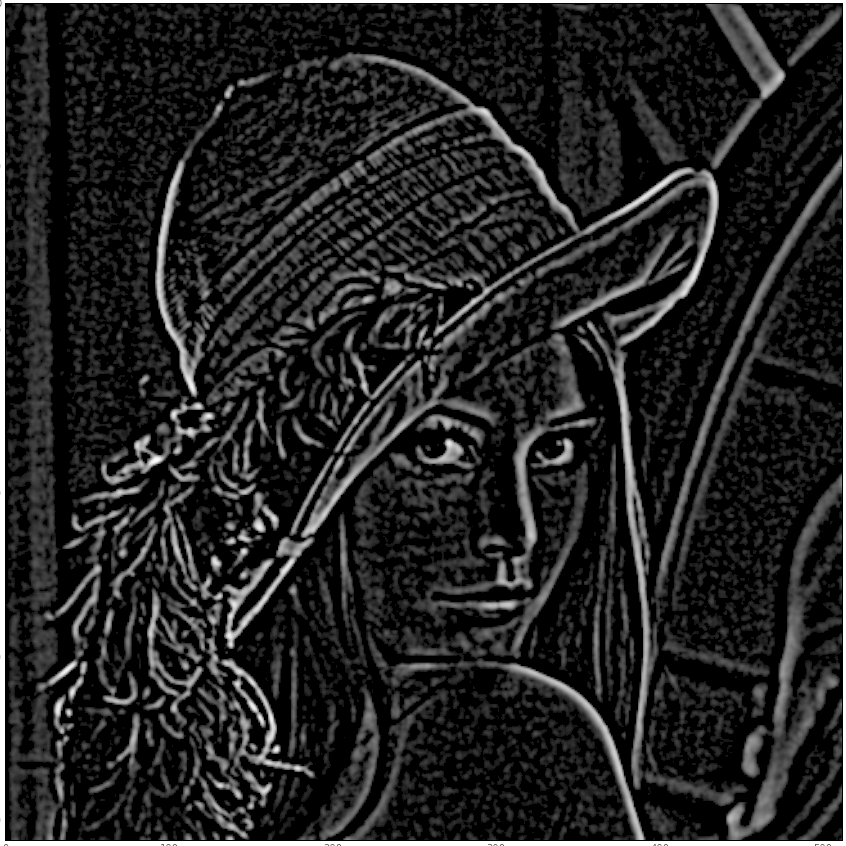
\includegraphics[width=\textwidth]{./Lena-midget_on}
    \caption{Layer 2}
    \label{pic-lena-M-ON}
  \end{subfigure}
  \begin{subfigure}[t]{0.32\textwidth}
    \vspace*{0.8em}
    \centering
    \captionsetup{justification=centering,margin=0.1cm}
    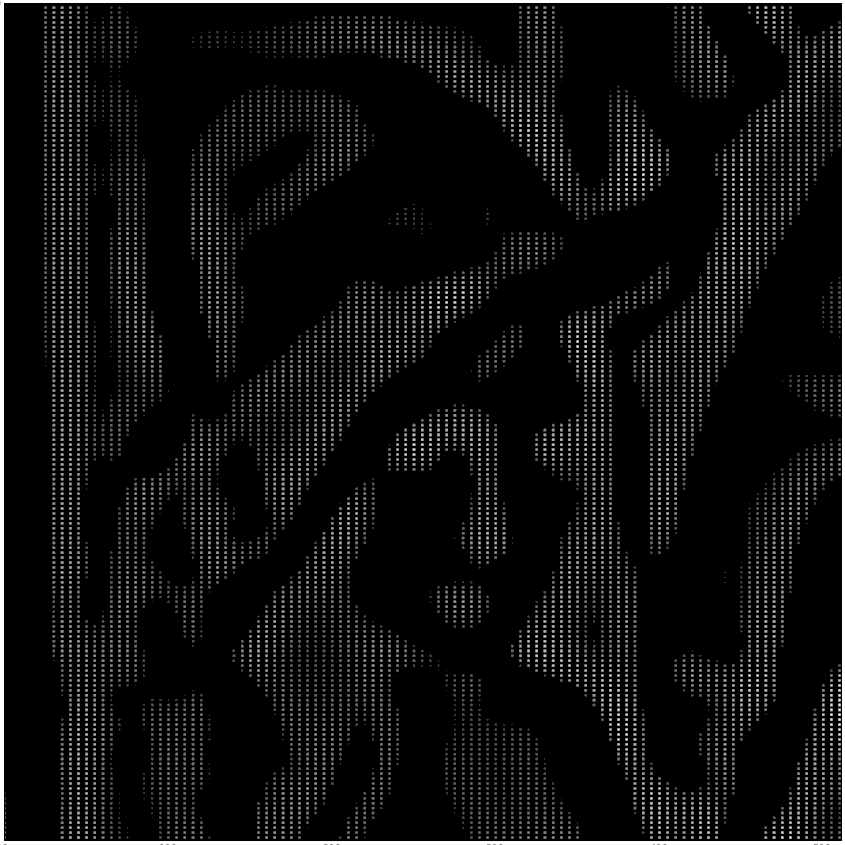
\includegraphics[width=\textwidth]{./Lena-parasol_off}
    \caption{Layer 3}
    \label{pic-lena-P-OFF}
  \end{subfigure}
  \begin{subfigure}[t]{0.32\textwidth}
    \vspace*{0.8em}
    \centering
    \captionsetup{justification=centering,margin=0.1cm}
    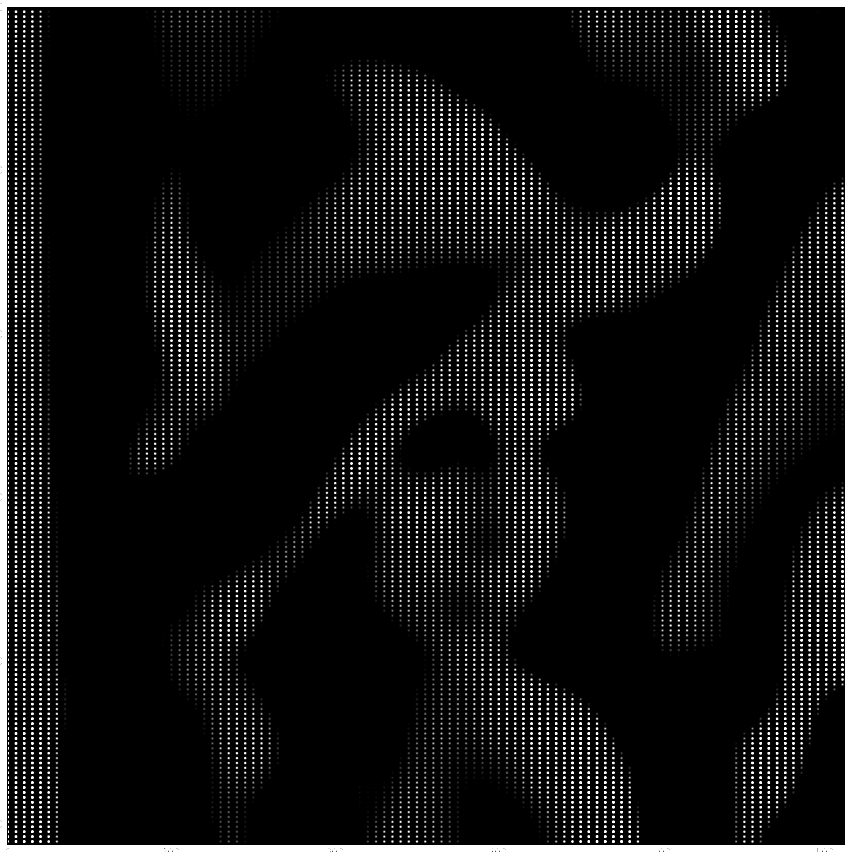
\includegraphics[width=\textwidth]{./Lena-parasol_on}
    \caption{Layer 4}
    \label{pic-lena-P-ON}
  \end{subfigure}
  \caption{Results of simulating ganglion cell layers (convolved images were enhanced for better contrast)}
  \label{fig-convolution-results}
\end{figure}

In order to check the validity of the generated spikes, a reconstruction procedure is employed (Equation \ref{eq:reconstruction}). Each coefficient in $C$ has an origin layer $w$, a value $c$ and a position ($k$, $l$). For all coefficients in $C$, the DoG kernel for layer $w$ will be weighed by the coefficient's value and be summed to the reconstructed image  $R$ at the coefficient's original position. The procedure is based on the assumption that the DoG are orthogonal basis. Figure \ref{pic-unfiltered-spikes} shows the result of the image reconstruction procedure without any redundancy correction applied.

\begin{equation}
  R(x,y) = \sum_{i}^{} \sum_{j}^{} \sum_{w}^{} C_{w}(i - x, j - y)DoG_{w}(i, j)
  \label{eq:reconstruction}
\end{equation}

\begin{figure}[hbt]
  \centering
  \begin{subfigure}[t]{0.3\textwidth}
    \centering
    \captionsetup{justification=centering,margin=0.1cm}
    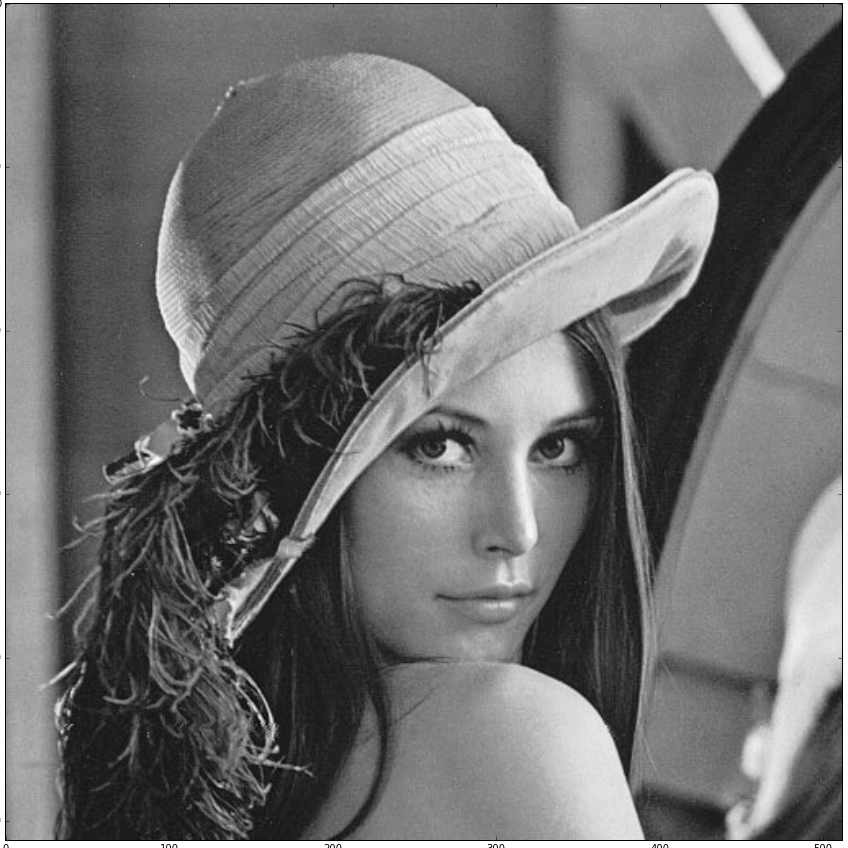
\includegraphics[width=\textwidth]{./Lena-gray}
    \caption{Original image}
  \end{subfigure}
  \begin{subfigure}[t]{0.3\textwidth}
    \centering
    \captionsetup{justification=centering,margin=0.1cm}
    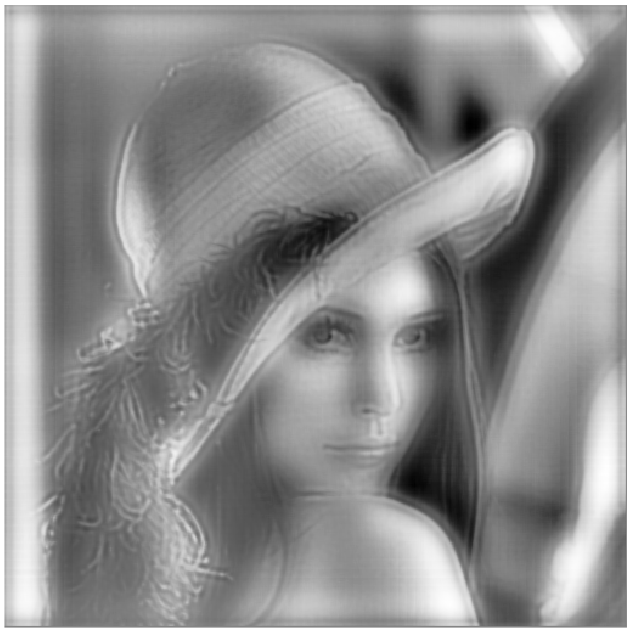
\includegraphics[width=\textwidth]{./final_results-unfiltered}
    \caption{100\% of raw spikes}
    \label{pic-unfiltered-spikes}
  \end{subfigure}
  \caption{Reconstruction results without overlap correction.}
\end{figure}

The eye is unlikely to provide unnecessary information to the brain, so it seems likely that redundant information is filtered out by the retina, perhaps by mutual inhibition.
It's still a matter of debate as to where, and by which cells, is lateral inhibition performed, it is most likely to happen in layers prior to the ganglion cell layer~\cite{eye-brain-vision-hubel1995}. 

The DoG kernels are only an approximately orthogonal basis, thus the resulting coefficients from the convolutions in Algorithm \ref{code-focal-conv} contain redundant information. That is, two neighbouring pixels might represent the same feature in the image. The main issue with this redundancy is that neighbouring coefficients might encode almost the same information with a similar value. Since the value provides the order of the spikes, this phenomenon will push other non-redundant and important coefficients into the later parts of the spike representation. In order to correct for redundancy, FoCal performs a second step (Algorithm \ref{code-focal-corr}).

\begin{algorithm}[htb]
  \caption{FoCal, Part 2}
  \label{code-focal-corr}
  \begin{algorithmic}
    \algrestore{bkbreak}
    \Procedure{Correction}{coeffs $C$, correlations $Q$}
    \State $N \leftarrow \emptyset$ \Comment{Corrected coefficients}
    \Repeat
    \State $m \leftarrow max(C)$
    \State $M \leftarrow M \cup m$
    \State $C \leftarrow C \setminus m$
    \ForAll{$ c \in C$} \Comment{Adjust all remaining c}
    \If{$Q(m, c) \neq 0$} \Comment{Adjust only near}
    \State $c \leftarrow c - m \times Q(m, c)$
    \EndIf
    \EndFor
    \Until{$C = \emptyset$}
    \State \textbf{return} $M$
    \EndProcedure
  \end{algorithmic}
\end{algorithm}

All the coefficients that where obtained from Algorithm \ref{code-focal-conv}, are put in a set $C$. For every step of the correction procedure, the maximum coefficient is searched and the surrounding pixels in each layer (Figure \ref{fig:focal2}) are adjusted according to the correlation due to overlap between the maximum coefficient's convolution kernel and the layer's kernel. The bold square in Figure \ref{fig:overlap} shows the overlap of two $3\times3$ kernels of neighbouring pixels, a similar overlap is considered for the interaction between layers.

\begin{figure}[htb]
  \centering
  \begin{subfigure}[t]{0.68\textwidth}
  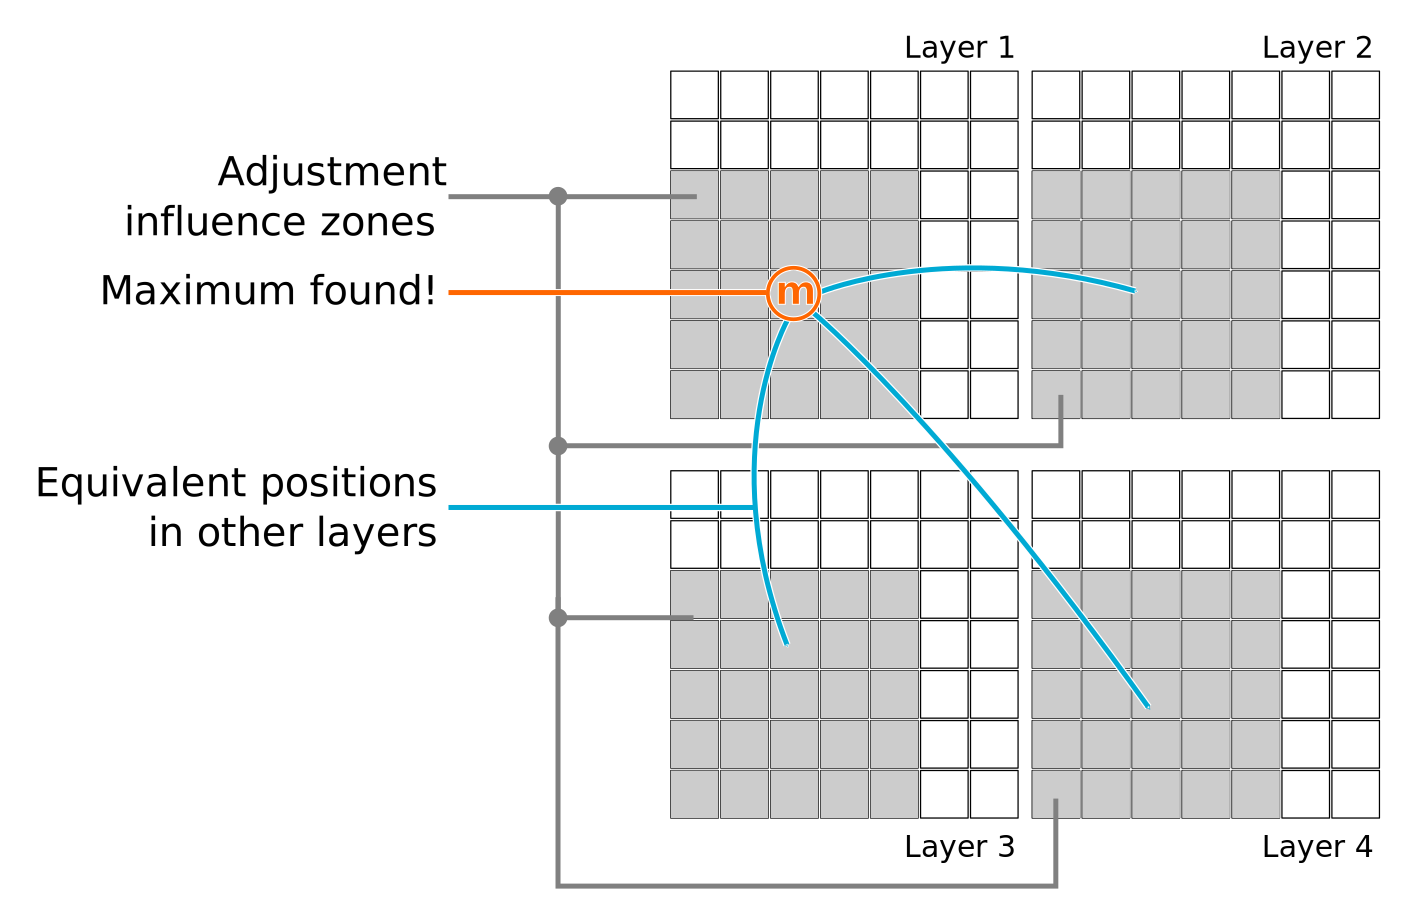
\includegraphics[width=\textwidth]{correction_adjustment}
  \caption{FoCal correction influence zones.}
  \label{fig:focal2}
  \end{subfigure}
  \hfill
  \begin{subfigure}[t]{0.29\textwidth}
  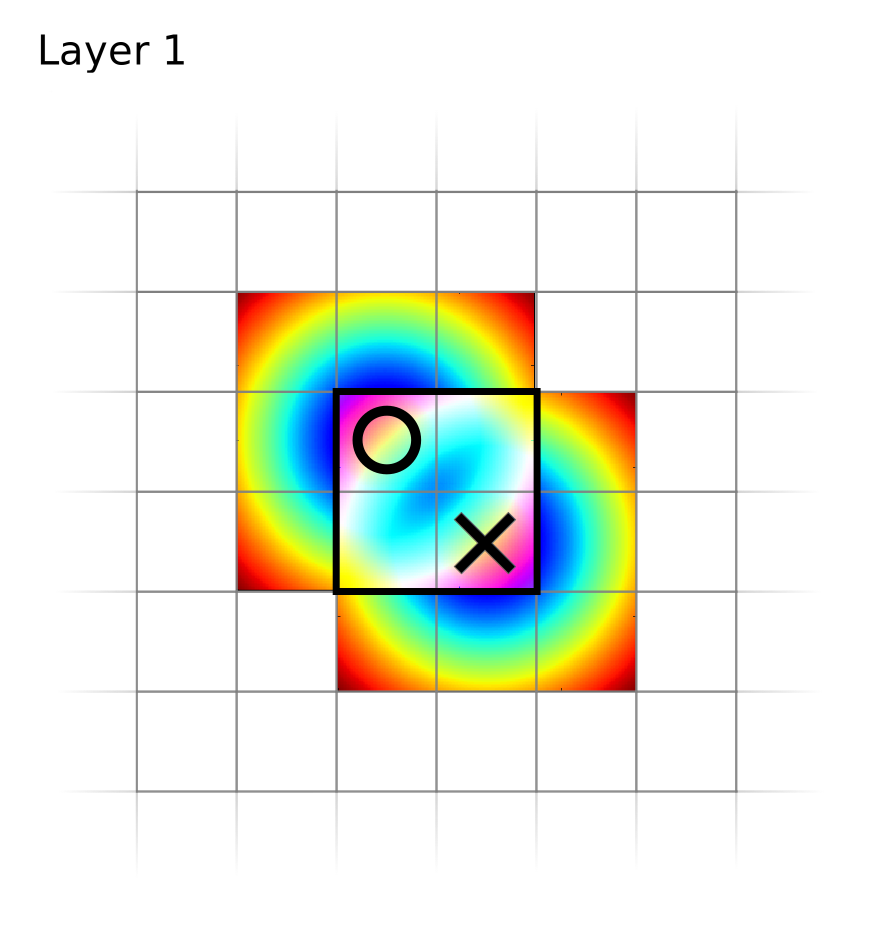
\includegraphics[width=\textwidth]{./coefficient_overlap}
  \caption{Kernel overlap}
  \label{fig:overlap}
  \end{subfigure}
\end{figure}

After this correction algorithm is applied, only non-redundant spikes are preserved, this results in a much better reconstruction (Figure \ref{pic-100pc-spikes}). Not only is it more visually pleasing, but the fidelity of the reconstruction has been tested quantitatively; another interesting result is that only 10\% of the spikes are needed to preserve 90\% of the visually important information~\cite{basab-thesis}.

\begin{figure}[hbt]
  \centering
  \begin{subfigure}[t]{0.3\textwidth}
    \centering
    \captionsetup{justification=centering,margin=0.1cm}
    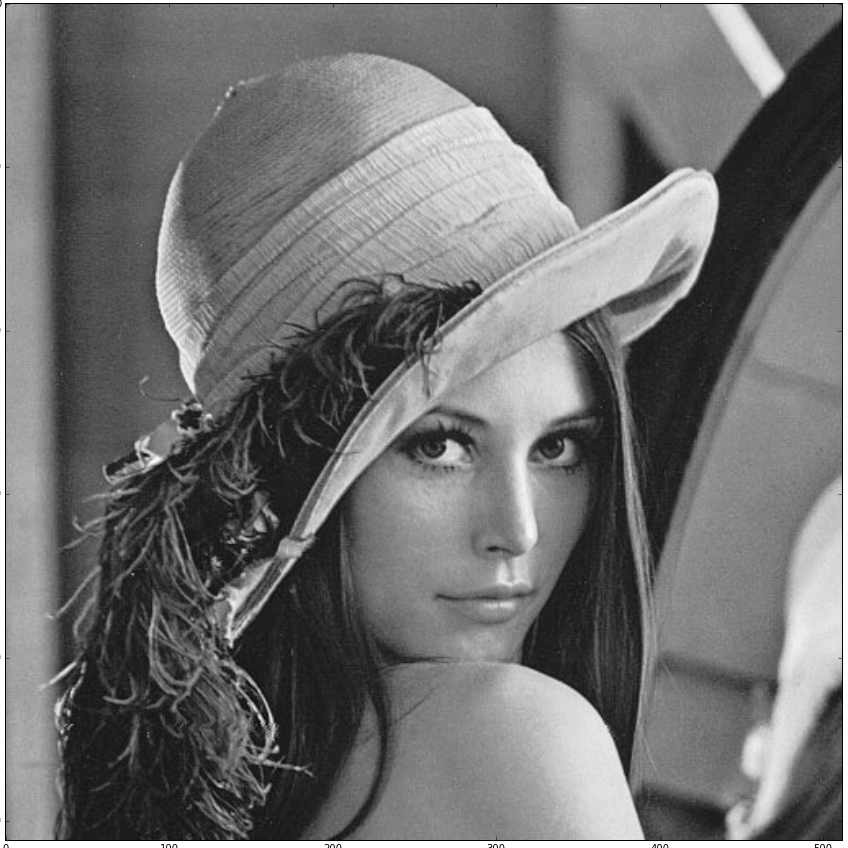
\includegraphics[width=\textwidth]{./Lena-gray}
    \caption{Original image}
    \label{pic-original-lena}
  \end{subfigure}
  \begin{subfigure}[t]{0.3\textwidth}
    \centering
    \captionsetup{justification=centering,margin=0.1cm}
    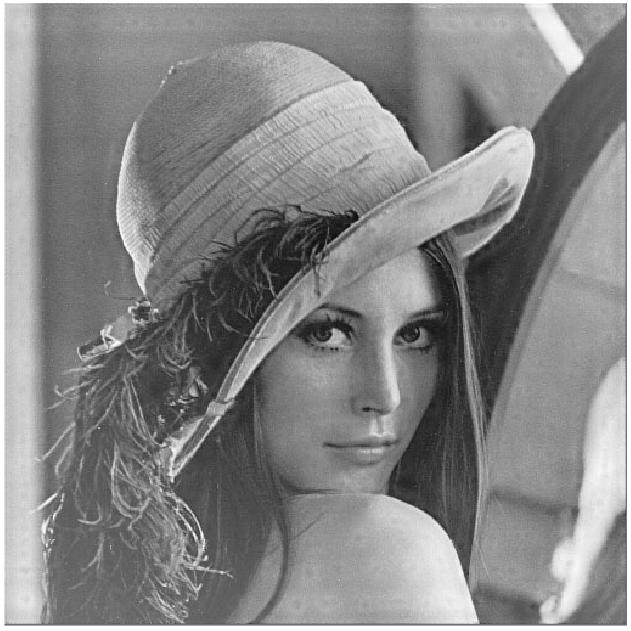
\includegraphics[width=\textwidth]{./final_results-focal-100}
    \caption{100\% of \emph{corrected} spikes}
    \label{pic-100pc-spikes}
  \end{subfigure}
  \begin{subfigure}[t]{0.3\textwidth}
    \centering
    \captionsetup{justification=centering,margin=0.1cm}
    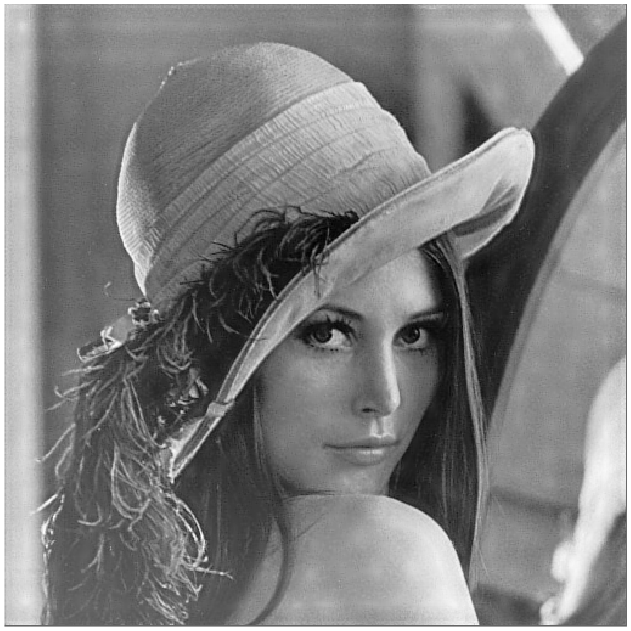
\includegraphics[width=\textwidth]{./final_results-focal-30pc}
    \caption{30\% of \emph{corrected} spikes}
    \label{pic-30pc-spikes}
  \end{subfigure}
  \caption{Results of reconstruction procedure}
  \label{fig-reconstruction}
  \vspace*{-10pt}
\end{figure}
\vspace*{0.5cm}

\hspace*{-0.65cm}\emph{Implementation details}\\[0.3cm]
Different ways of applying convolutions to images on a GPU where implemented and evaluated. First, the \textbf{naïve approach}, implies a discrete convolution with the full 2D kernels. Since we are using square kernels, this means $N^2 \times W \times H$ operations for a $W\times H$ image using a kernel of width $N$. As expected, performance drops quickly as kernel size increases and the largest one ($243\times243$ elements) requires more resources than the GPU's \emph{constant memory}\footnote{A special type of global memory that has faster access times.} can provide (240 vs 64 KBytes). This results in execution errors that may only be fixed using memory with greater latency to store the convolution kernel. 


The second method of performing a 2D DoG convolution on an image is to rely on \textbf{kernel separability}. A convolution kernel $K$ is said to be \emph{separable} if $K = K_{1} \ast K_{2} \dots K_{n}$. Gaussian kernels are separable (Eq. \ref{eq:Gto1D}). 

\begin{equation}
  G \ast I = \sum_{i} \sum{j} e^{x^2 + y^2}I(i, j)  = \sum{j} e^{y^2}\left[ \sum_{i} e^{x^2}I(i, j) \right] = G_V \ast ( G_H \ast I)
  \label{eq:Gto1D}
\end{equation}

Fortunately a DoG is merely the subtraction of them (Eq. \ref{eq:DoG2G}).
\vspace*{0.5cm}

\begin{equation}
O = I \ast DoG = I \ast G_{c} - I \ast G_{s}
\label{eq:DoG2G}
\end{equation}

Applying the algebraic properties of convolutions and the fact that Gaussian kernels are separable, the full 2D DoG convolution can be performed using four 1D separated ones (Eq. \ref{eq:DoGto1D}).

\begin{equation}
O = I \ast DoG = G_{v,c} \ast G_{h,c} \ast I - G_{v,s} \ast G_{h,s} \ast I 
\label{eq:DoGto1D}
\end{equation}

The main advantage of the separated kernel approach is a reduction of the number of operations needed ($4N\times W \times H$). The convolution with a $3\times 3$ kernel is an exception, in this case there are 12 operations versus the 9 needed for the naïve approach.


The last approach tried, \emph{Tiled Convolution} was reported by Advanced Micro Devices (AMD)~\cite{tiled-convolution}. They only present kernels of size $3\times3$, but we have an $11\times11$ convolution working. The algorithm is based on separable convolution. The main advantage is that results from the horizontal 1D convolution are reused to calculate the final result (Figure~\ref{fig:c2s:tiled-conv}). Convolutions for larger kernels are not optimal with this method due to local memory size.

\begin{figure}[h]
  \begin{center}
    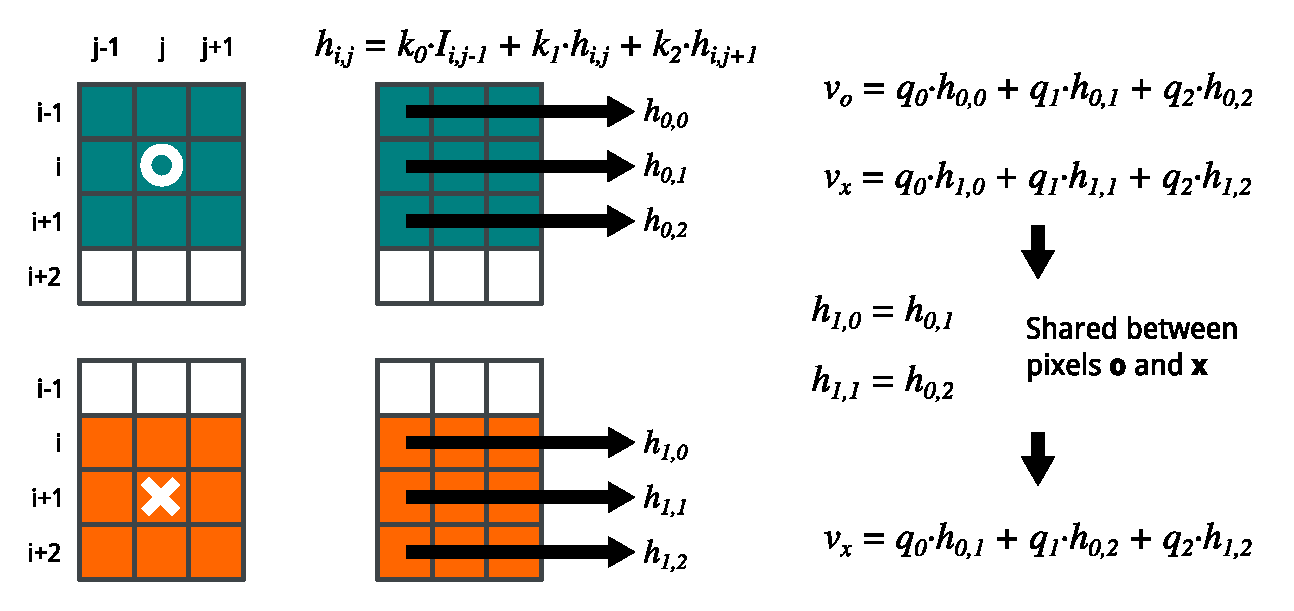
\includegraphics[width=0.8\textwidth]{tiled-conv}
    \caption{Tiled convolution, calculations are shared by vertical neighbours.}
    \label{fig:c2s:tiled-conv}
  \end{center}
\end{figure}

Convolution alone is a compute intensive task and we obtain about 12 frames-per-second (FPS) on videos with $640\times360$ resolution and 8-bit grey-scale pixels. Encoding was carried out using a desktop computer running 64-bit GNU/Linux and OpenCL 1.1. The system has a Core i5-4570 4-core CPU @ 3.20~GHz processor with 8~GBytes of 64-bit DDR3 RAM @ 1600~MHz and a GeForce GT 720 GPU with 192 CUDA cores @ 797~MHz, 1~GBytes of 64-bit DDR3 RAM @ 1800~MHz. The performance of convolution in GPUs is mainly bound by memory transfers, even if the information is reused. %\\

\begin{table}[hbt]
  \begin{center}
    \caption{Convolution performance comparison.}
    \bgroup
    \def\arraystretch{1.4}
    \begin{tabular}{l c c c c}
      &
      \begin{minipage}{2cm}\centering Layer 0\vspace*{0.1cm}\end{minipage} & 
      \begin{minipage}{2cm}\centering
        Layer 1\vspace*{0.1cm}\end{minipage}& 
      \begin{minipage}{2cm}\centering
        Layer 2\vspace*{0.1cm}\end{minipage}& 
      \begin{minipage}{2cm}\centering
        Layer 3\vspace*{0.1cm}\end{minipage}\\
      \hline 
      
      Naïve     & $0.0009 s$ & $0.0031 s$ & $0.0587 s$ & N/A$^{1,2}$ \\ 
      Separated & $0.0021 s$ & $0.0055 s$ & $0.0172 s$ & $0.0472 s$ \\ 
      % x, y, 0.01756, 0.04500
      Tiled     & $0.0009 s$ & $0.0044 s$ & $0.1643 s$ & N/A$^2$\\
    \end{tabular} 
    \egroup
    {
      \footnotesize 
      \begin{center}
        $^1$ Unable to fit convolution kernel into constant memory.\\
        $^2$ Unable to compile OpenCL code.
      \end{center}
    }
  \end{center}
  \vspace*{-5pt}
\end{table}

Correcting the spikes for redundancy is a highly time consuming task which
might be better suited for event-based programming, such as the one found on 
the SpiNNaker platform. The main advantage of this encoding is that visually important information is retained, that is, an image may be reconstructed from the spike trains. 



\subsubsection{A dynamic vision sensor emulator}

Dynamic vision sensors (DVS) have changed the way visual information is acquired, they sense temporal contrast differences in the $\mu s$ scale. The main issue with these devices is that they are still in development and may be expensive~\cite{aer-retina-bernabe,dvs-zurich}. The purpose of this encoder is to provide an output similar to that of a DVS, but using a camera as a sensor.

The main advantage is that no specialized hardware is needed and the operations are simple enough that any recent computer should be able to perform them in real time, although a full reconstruction of the image is not possible as was the case for the foveal pit model.

Spatial contrast changes are detected through a convolution using DoG kernels, similar to the ones used in the foveal pit-based encoder. Contrast changes in time are detected by subtracting the previous frame from the current, both of them were previously convolved. If the absolute value of the difference (on a per-pixel basis) is higher than a certain threshold, the neuron on the pixel location is considered to have emitted an action potential. 
%current and past frames ? centre - current / surround - past

Threshold values are independent for each pixel and change according simple rules. If a pixel did not spike, the threshold is decreased to account for light accumulating on the sensor; otherwise the threshold is increased to emulate a refractory period of cells (Figure~\ref{fig:c2s:threshold_behaviour}).

\begin{figure}[h]
  \begin{center}
    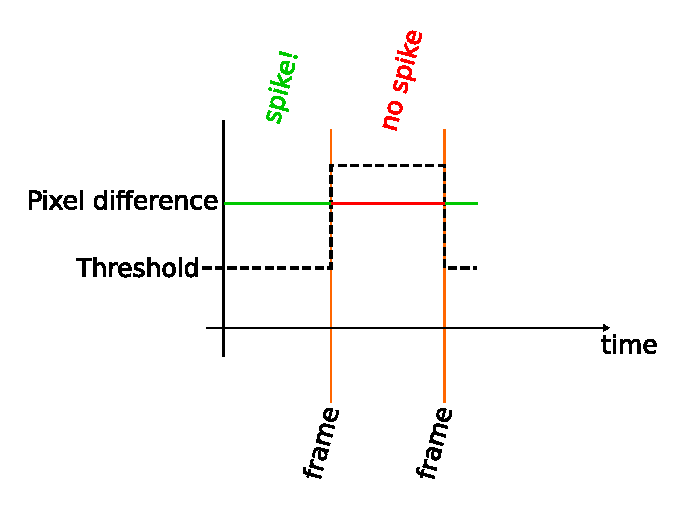
\includegraphics[width=0.55\textwidth]{DVSemu}
    \caption{Adaptive threshold behaviour.}
    \label{fig:c2s:threshold_behaviour}
  \end{center}
\end{figure}
\newpage
Once the spiking pixels have been calculated, they are sorted to generate a spike-time encoding. The hypothesis here is that the larger the contrast change, the sooner a cell would spike. A sample of the output is shown in Figure~\ref{fig:c2s:dvs-emu-output}.

\begin{figure}[h]
  \begin{center}
    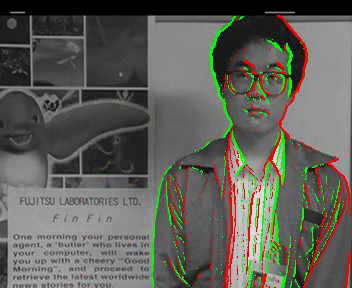
\includegraphics[width=0.6\textwidth]{dvs-emu-img}
    \caption{Output of the DVS emulator, red pixels indicate a negative change in contrast; a positive alteration is illustrated by green pixels.}
    \label{fig:c2s:dvs-emu-output}
  \end{center}
\end{figure}

The procedure can perform at about 25 frames per second using an OpenCL back-end (using the same hardware setup previously described). Although 
it's currently a good approximation, more research on this algorithm is needed 
to better approximate the original devices.

